% =========================================================================
% Capítulo 1: Cinemática
% Tema 01: Coordenadas cilíndricas
% Problema 09: Hélice circular
% =========================================================================
\subsubsection{Hélice circular}

Una partícula $P$ se desplaza siguiendo una trayectoria helicoidal sobre la superficie lateral de un cilindro vertical de radio $R$, como se muestra en la Figura \ref{fig:helice_3d}. La hélice mantiene un ángulo de inclinación constante $\phi$ respecto al plano horizontal. Utilizando coordenadas cilíndricas $(r, \theta, z)$, donde el eje $z$ coincide con el eje del cilindro, realice lo siguiente:

\begin{enumerate}
    \item Defina los marcos de referencia y los sistemas de coordenadas (fijos y móviles) adecuados para describir el movimiento tridimensional.
    \item Determine el vector posición de la partícula $P$ respecto al origen $O$ situado en el centro de la base inferior.
    \item Obtenga la velocidad y la aceleración de la partícula $P$ respecto a un marco inercial.
    \item Calcule la longitud de arco recorrida por la partícula $P$, si en el inicio $\theta(0)=0$.
\end{enumerate}

\begin{figure}[!ht]
    \centering
    \begin{tikzpicture}[>=Latex, x={(1cm,-0.2cm)}, y={(1cm,0.1cm)}, z={(0cm,1cm)}, scale=2]
        % --- Parámetros Geométricos ---
        \def\R{1.5}      % Radio
        \def\H{3.0}      % Altura
        \def\pitch{0.4}  % Paso de la hélice (proporcional a tan(phi))
        \def\pAng{120}   % Ángulo theta para la posición de P

        % --- 1. Ejes de Coordenadas ---
        \draw[->, thin, gray] (0,0,0) -- (2.5,0,0) node[right] {$x$};
        \draw[->, thin, gray] (0,0,0) -- (0,2.5,0) node[above right] {$y$};
        \draw[->, thick] (0,0,0) -- (0,0,3.5) node[above] {$z$};
        \node[below left] at (0,0,0) {$O$};

        % --- 2. Cilindro (Estructura) ---
        % Base inferior (parte trasera oculta)
        \draw[dashed, gray] (\R,0,0) arc (0:180:\R);
        % Base inferior (parte delantera)
        \draw[thick] (\R,0,0) arc (0:-180:\R);
        
        % Líneas laterales
        \draw[gray!50] (-\R,0,0) -- (-\R,0,\H);
        \draw[gray!50] (\R,0,0) -- (\R,0,\H);

        % Tapa superior (Elipse)
        \draw[thick, fill=gray!5, fill opacity=0.3] (0,0,\H) circle [radius=\R];

        % --- 3. Trayectoria Helicoidal ---
        % Hélice trasera (punteada)
        \draw[blue!50, dashed, domain=0:pi, samples=50, variable=\t] 
            plot ({\R*cos(\t r)}, {\R*sin(\t r)}, {\pitch*\t});
        \draw[blue!50, dashed, domain=2*pi:2.5*pi, samples=50, variable=\t] 
            plot ({\R*cos(\t r)}, {\R*sin(\t r)}, {\pitch*\t});

        % Hélice delantera (continua)
        \draw[ultra thick, blue!80!black, domain=pi:2*pi, samples=50, variable=\t] 
            plot ({\R*cos(\t r)}, {\R*sin(\t r)}, {\pitch*\t});
        \draw[ultra thick, blue!80!black, domain=-0.5*pi:0, samples=50, variable=\t] 
            plot ({\R*cos(\t r)}, {\R*sin(\t r)}, {\pitch*\t});

        % --- 4. Partícula P y Parámetros ---
        % Coordenadas de la partícula
        \pgfmathsetmacro{\Px}{\R*cos(\pAng)}
        \pgfmathsetmacro{\Py}{\R*sin(\pAng)}
        \pgfmathsetmacro{\Pz}{\pitch*\pAng*pi/180}
        
        \coordinate (P) at (\Px, \Py, \Pz);
        \coordinate (Pbase) at (\Px, \Py, 0);

        % Líneas de proyección
        \draw[dashed, thin] (0,0,0) -- (Pbase);
        \draw[dashed, thin] (Pbase) -- (P);
        \draw[dashed, thin] (P) -- (0,0,\Pz);

        % Partícula
        \filldraw[shading=ball, ball color=black] (P) circle (1.2pt) node[above right] {$P$};

        % Radio R y Ángulo Theta
        \draw[<->] (0,0,0) -- ({\R*cos(210)}, {\R*sin(210)}, 0) node[midway, below left] {$R$};
        \draw[->] (0.5,0,0) arc (0:\pAng:0.5);
        \node at (0.24, 0.32, 0) {$\theta$};

        % Ángulo de inclinación Phi
        \begin{scope}[shift={(1.5,0)}]
            \draw[dashed] (0,0,0) -- (0, 1.2, 0);
            \draw[->] (0, 0.4, 0) arc (20:90:0.4);
            \node[right] at (0.4, 0, 0.3) {$\phi$};
        \end{scope}


    \end{tikzpicture}
    
    \caption{Análisis tridimensional de la cinemática de una partícula en trayectoria helicoidal.}
    \label{fig:helice_3d}
\end{figure}

% --- SOLUCIÓN ---------------------------------------------------------------
\begin{solucion}{Hélice circular}
\textbf{Marcos de referencia y Sistemas de Coordenadas}\\
Lo primero, como en todo ejercicio, es definir los marcos de referencia.
\begin{itemize}
    \item $\mathcal{N}$ El suelo $\longrightarrow\{\vec{E}_x;\vec{E}_y;\vec{E}_z\}$
    \item $\mathcal{A}$ Centro $O$ - proyección de $P$ $\longrightarrow\{\vec{e}_r;\vec{e}_\theta;\vec{e}_z\}$
\end{itemize}

\begin{center}
\begin{tikzpicture}[>=Stealth, scale=3]
    % --- SISTEMAS DE COORDENADAS ---
    \def\angOmega{55} % Ángulo de rotación
    \draw[->] (-1.2,0) -- (1.3,0);
    \draw[->] (0,-1.2) -- (0,1.3);
    \draw (0,0) circle (1);
    % Base fija (azul)
    \draw[->, blue, thick] (0,0) -- (0.8,0) node[anchor=north] {$\vec{E}_x$};
    \draw[->, blue, thick] (0,0) -- (0,0.8) node[anchor=east] {$\vec{E}_y$};
    % Base móvil (verde)
    \draw[->, green!60!black, thick] (0,0) -- (\angOmega:0.8) node[above left] {$\vec{e}_r$};
    \draw[->, green!60!black, thick] (0,0) -- (\angOmega+90:0.8) node[anchor=south east] {$\vec{e}_\theta$};
    % --- PUNTOS ---
    \fill[gray] (\angOmega:1) circle (2pt);
    \node[anchor=north west] at (\angOmega:1) {$P$};
    % --- ÁNGULO ---
    \draw (0.4,0) arc (0:\angOmega:0.4);
    \node at (25:0.5) {$\theta$};
    % Eje z saliendo de la página
    \draw[fill=white] (0,0) circle (0.08);
    \fill (0,0) circle (1pt);
    \node[anchor=north east] at (-0.05,-0.05) {$\vec{E}_z = \vec{e}_z$};
\end{tikzpicture}
\end{center}
\begin{equation*}
\begin{split}
    \vec{e}_r&=\cos(\theta)\vec{E}_x+\sin(\theta)\vec{E}_y\\
    \vec{e}_\theta&=-\sin(\theta)\vec{E}_x+\cos(\theta)\vec{E}_y\\
    \vec{e}_z&=\vec{E}_z
\end{split}
\end{equation*}

\subsubsection*{Cinemática de la partícula}
\textbf{Posición}\\
Como siempre, para obtener la velocidad de algún punto respecto a un marco de referencia inercial, hay que partir de la posición; en este caso la de la partícula $P$ es
$$\vec{r}_P=r\vec{e}_r+z\vec{e}_z$$
Y necesitamos encontrar $z$ en términos de cosas conocidas; para esto ocupamos el ángulo de inclinación $\phi$. Si nos vamos al borde del cilindro tenemos un triángulo en el cual el cateto inferior corresponde a la distancia recorrida en la dirección angular (también se puede ver diferencialmente como un pequeño cambio, la distancia recorrida es $Rd\theta$), que se puede representar como $R\theta$ donde recordemos que $\theta$ es el ángulo en radianes. Ahora nos falta el otro cateto, que corresponde a cuánto ha subido la partícula ($z$) respecto a cuánto se ha recorrido ($R\theta$).
\begin{center}
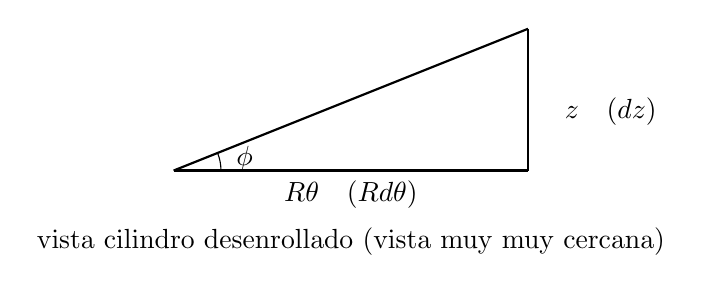
\begin{tikzpicture}[scale=1.5]
    % --- TRIÁNGULO (cilindro desenrollado) ---
    \draw[thick] (0,0) -- (3,1.2); % hipotenusa
    \draw[thick] (0,0) -- (3,0);   % base
    \draw[thick] (3,0) -- (3,1.2); % lado
    % --- ÁNGULO PHI ---
    \draw[dashed] (0,0) -- (0.8,0);
    \draw[dashed] (0,0) -- (0.8,0.32);
    \draw[-] (0.4,0) arc (0:21:0.4);
    \node at (0.6,0.1) {$\phi$};
    % --- ETIQUETAS ---
    \node at (1.5,-0.6) {vista cilindro desenrollado (vista muy muy cercana)};
    \node at (3.7,0.5) {$z\quad(dz)$};
    \node at (1.5,-0.2) {$R\theta \quad(Rd\theta)$};
\end{tikzpicture}
\end{center}
$$\tan(\phi)=\dfrac{z}{R\theta}=\dfrac{dz}{Rd\theta}\longrightarrow z=R\theta\tan(\phi)$$

\patotruco{Como $\phi$ es constante, $z$ queda amarrado a $\theta$ y todo el movimiento depende de una única función $\theta(t)$. Además, en cilíndricas la base se deriva directo: $\dot{\vec{e}}_r=\dot\theta\vec{e}_\theta$ y $\dot{\vec{e}}_\theta=-\dot\theta\vec{e}_r$ (el ``trucazo'', que es el teorema del transporte ya resuelto).}

\textbf{Velocidad}\\
Como se sabe, la velocidad es la derivada temporal de la posición desde un punto fijo.
$$\marc{\vec{v}_P}{N}=\der{\vec{r}_{P}}{N}=\der{(R\vec{e}_r+R)}{N}= R\der{\vec{e}_r}{N}+R\dot\theta\tan(\phi)\vec{e}_z$$
En este caso no es necesario utilizar teorema del transporte porque usamos el trucazo.\\
Derivadas temporales de $\vec{e}_r$ y $\vec{e}_\theta$
$$\transport{\vec{e}_r}{N}{A}=\dot\theta\vec{e}_z\times\vec{e}_r=\dot\theta\vec{e}_\theta $$
$$\transport{\vec{e}_\theta}{N}{A}=\dot\theta\vec{e}_z\times\vec{e}_\theta=-\dot\theta\vec{e}_r $$
y finalmente
$$\marc{\vec{v}_P}{N}=R\dot\theta\vec{e}_\theta+R\dot\theta\tan(\phi)\vec{e}_z$$

\textbf{Aceleración}\\
Al igual que antes podemos simplemente derivar la velocidad para obtener la aceleración.
$$\marc{\vec{a}_P}{N}=\der{\marc{\vec{v}_P}{N}{}}{N}{}=\der{\left(R\dot\theta\vec{e}_\theta+R\dot\theta\tan(\phi)\vec{e}_z\right)}{N}{}=(-R\dot\theta^2)\vec{e}_r+ R\ddot\theta\vec{e}_{\theta}+R\ddot\theta\tan(\phi)\vec{e}_z$$

\textbf{Longitud de arco}\\
La longitud de arco se define como la distancia que recorre la partícula en un lapso de tiempo. Para esto es muy útil saber cuánto recorre en un tiempo ínfimo y se multiplica por el tiempo, así se suma
$$ds=\|\vec{v}_p\|dt\longrightarrow s-s_0=\int\sqrt{R^2\dot\theta^2(1+\tan^2(\phi))}=\int R\dot\theta\sec(\phi)dt$$
Hacemos un cambio de variable, asumiendo que $\theta$ es solo creciente o solo decreciente, es decir, $\dot\theta$ no varía de signo
$$s=\int_{t_0}^t R\dot\theta\sec(\phi)dt\longrightarrow\int_{\theta_0}^\theta R\sec\phi \,\text{d}\theta=R(\theta-\theta_0)\sec(\phi)$$
\respuesta{$\displaystyle s=R\,\theta\sec(\phi)\quad(\theta_0=0)$}
\end{solucion}
